\documentclass[11pt]{article}
\usepackage{amsmath, amssymb, amsthm}
\usepackage[margin=1in]{geometry}
\usepackage{booktabs}
\usepackage{graphicx}

\title{Predicting plateau-breaking angles from feature geometry}
\author{Francisco Ferreira da Silva}
\date{\today}

\begin{document}
\maketitle

\section{Setup}

Consider a transformer with residual stream dimension $n$.
We assume the model has $m \gg n$ features, represented by unit vectors $\{f_1, \ldots, f_m\}$ in $\mathbb{R}^n$.
We further assume these features are approximately uniformly spread on the unit sphere, as this minimizes interference between features.

Real activations of large-enough transformers resist perturbations, a phenomenon known as activation plateaus.
The same does not hold for randomly sampled points in activation space (random or synthetic activations), under various sampling conditions.
This holds across a wide range of model sizes and families, does not occur in untrained large language models, and sharpens as models get deeper and as training progresses.

Activation plateaus can be elicited as follows.
We perturb an activation $\mathbf{a}$ at layer $L$ by rotating it toward a unit direction $\mathbf{d}$ by angle $\theta$, keeping the norm fixed.
We then forward-pass to a later layer and measure the downstream response (e.g., cosine distance between clean and perturbed activations).
We define the \emph{plateau-breaking angle} $\theta_{\mathrm{break}}(\mathbf{d})$ as the perturbation angle at which the downstream response exceeds some threshold $\epsilon$.
Empirically, we observe that perturbation along known features breaks the plateau at a small angle $\theta_1$, and that perturbation along random directions breaks the plateau at a much larger angle $\theta_{\mathrm{rand}}$.
Note that this suggests an unsupevised method for feature finding: features are directions with $\theta_{\text{break}} \ll \theta_{\mathrm{rand}}$\footnote{This is conceptually similar to MELBO.}, which can be used to estimate $\theta_1$.

One explanation for this difference is that plateaus are a form of learned error correction.
A random perturbation decomposes into many features, each receiving only a small share of the total perturbation magnitude.
If we assume the model corrects perturbations falling below some per-feature threshold, the plateau persists until the perturbation angle is large enough that at least one feature receives a perturbation exceeding its threshold.
On the other hand, perturbation along a feature concentrates all magnitude into it, exceeding the threshold at a much smaller angle.

This motivates a simple quantitative model: the plateau breaks when the most-aligned feature receives enough perturbation magnitude to exceed its error-correction threshold.
We want to predict $\theta_{\mathrm{rand}}$ from $\theta_1$, $n$, and $m$.
Under our model, $\mathbf{d}$ breaks the plateau when
\begin{equation}
    \max_i |\langle \mathbf{d}, f_i \rangle| \cdot \sin(\theta) \geq \sin(\theta_1),
\end{equation}
where $\sin(\theta_1)$ is the per-feature magnitude required to break the plateau, calibrated from perturbations along known features.\footnote{Which can, for example, be found with unsupervised methods along the lines of what we suggested above.}

Define the maximum alignment of $\mathbf{d}$ with the feature set:
\begin{equation}
    \alpha(\mathbf{d}) = \max_i |\langle \mathbf{d}, f_i \rangle|.
\end{equation}
Then the predicted breaking angle for direction $\mathbf{d}$ is
\begin{equation}
    \theta_{\mathrm{break}}(\mathbf{d}) = \arcsin\!\left(\frac{\sin(\theta_1)}{\alpha(\mathbf{d})}\right),
\label{eq:predicted_break}
\end{equation}
provided $\alpha(\mathbf{d}) \geq \sin(\theta_1)$.
If that's not the case, the single-feature model predicts no breaking.
For unit vectors sampled uniformly at random $\mathbf{v} \in \mathbb{R}^n$ and a fixed unit vector $f$, the inner product $\langle \mathbf{v}, f \rangle$ has variance $1/n$.
For large $n$, the distribution is approximately $\mathcal{N}(0, 1/n)$.\footnote{This is a good approximation for $n>20$. For ChessGPT, $n=512$ and this is essentially exact.}
Since we assume the plateau breaks when the most-aligned feature exceeds its threshold and that we have $m$ features, we need the expected value of $\max_{i=1}^{m} |\langle \mathbf{v}, f_i \rangle|$ over all $m$ features.
Using the standard extreme value result for Gaussians:
\begin{equation}
    \mathbb{E}\!\left[\max_{i=1}^{m} |\langle \mathbf{v}, f_i \rangle|\right] \approx \sqrt{\frac{2 \ln m}{n}}.
\end{equation}
Substituting into Equation~\eqref{eq:predicted_break}, we get an expression for the plateau-breaking angle when perturbing along random directions:
\begin{equation}
    \theta_{\mathrm{rand}} \approx \arcsin\!\left(\sin(\theta_1) \cdot \sqrt{\frac{n}{2 \ln m}}\right).
\label{eq:plateau_breaking_rand}
\end{equation}

\section{Example Application}
We now consider a concrete example for which we have empirical data.
ChessGPT is a 16-layer transformer with 50M parameters that exhibits activation plateaus.
It has residual dimension $n=512$.
Via MELBO-like unsupervised feature discovery methods, we have found that there exist directions for which the plateau-breaking angle is $\theta \approx 5.5^\circ$.
Recall that the expected maximum alignment of a uniformly sampled random direction with a feature is given by:
\begin{equation}
\alpha_{\text{rand}} = \sqrt{\frac{2 \ln m}{512}},
\end{equation}
with $m$ being the total number of features.
While we do not have ground truth for the total number of features ChessGPT has, it is typically assumed that transformers have 10 to 100 times more features than they have dimensions.
Using Equation~\eqref{eq:plateau_breaking_rand}, we show in Table~\ref{tab:angles_rand_chess} the expected plateau-breaking angle for random directions as a function of the assumed number of features $m$.
\begin{table}[!ht]
\centering
\begin{tabular}{@{}ccc@{}}
    \toprule
    $m$ & $\alpha_{\mathrm{rand}}$ & $\theta_{\mathrm{rand}}$ (predicted) \\
    \midrule
    1{,}000   & 0.165 & $36^\circ$ \\
    5{,}000   & 0.184 & $31^\circ$ \\
    10{,}000  & 0.191 & $30^\circ$ \\
    20{,}000  & 0.198 & $29^\circ$ \\
    50{,}000  & 0.207 & $28^\circ$ \\
    \bottomrule
\end{tabular}
\caption{Random direction plateau-breaking angles under different assumed numbers of features for the 512-dimensional ChessGPT model, under a single-feature plateau-breaking angle of $\approx 6^\circ$.}
\label{tab:angles_rand_chess}
\end{table}

\subsection{Subspace prediction}
Suppose we have found $k$ orthogonal features spanning a subspace $U$ of dimension $k$.
Consider a random unit vector $\mathbf{v}$ drawn uniformly from $U$.
Its projection onto any of the $k$ features $f_i \in U$ has variance $1/k$, giving expected max alignment $\sqrt{2 \ln k / k}$.
Its projection onto any of the remaining $m - k$ features $f_j \notin U$ has expected squared magnitude $\|f_{j,U}\|^2 / k$, where $\mathbb{E}[\|f_{j,U}\|^2] \approx k/n$ for uniformly spread features, giving variance $\approx 1/n$, the same as for fully random directions.

The in-subspace contribution dominates when
\begin{equation}
    \sqrt{\frac{2 \ln k}{k}} > \sqrt{\frac{2 \ln(m - k)}{n}},
\end{equation}
which holds when $k \ll n$ (i.e., we have found far fewer features than the residual dimension).
In this regime, the predicted breaking angle for random-in-subspace directions is
\begin{equation}
    \theta_{\mathrm{sub}} \approx \arcsin\!\left(\sin(\theta_1) \cdot \sqrt{\frac{k}{2 \ln k}}\right).
    \label{eq:plateau_breaking_sub}
\end{equation}
For ChessGPT with $k = 25$ features:
\begin{equation}
    \alpha_{\mathrm{sub}} = \sqrt{\frac{2 \ln 25}{25}} \approx 0.51, \qquad
    \theta_{\mathrm{sub}} = \arcsin\!\left(\frac{\sin(5.5^\circ)}{0.51}\right) \approx 11^\circ.
\end{equation}

\subsection{Empirical validation}
Figure~\ref{fig:subspace_vs_random} shows all three regimes for ChessGPT.
\begin{figure}[!ht]
    \centering
    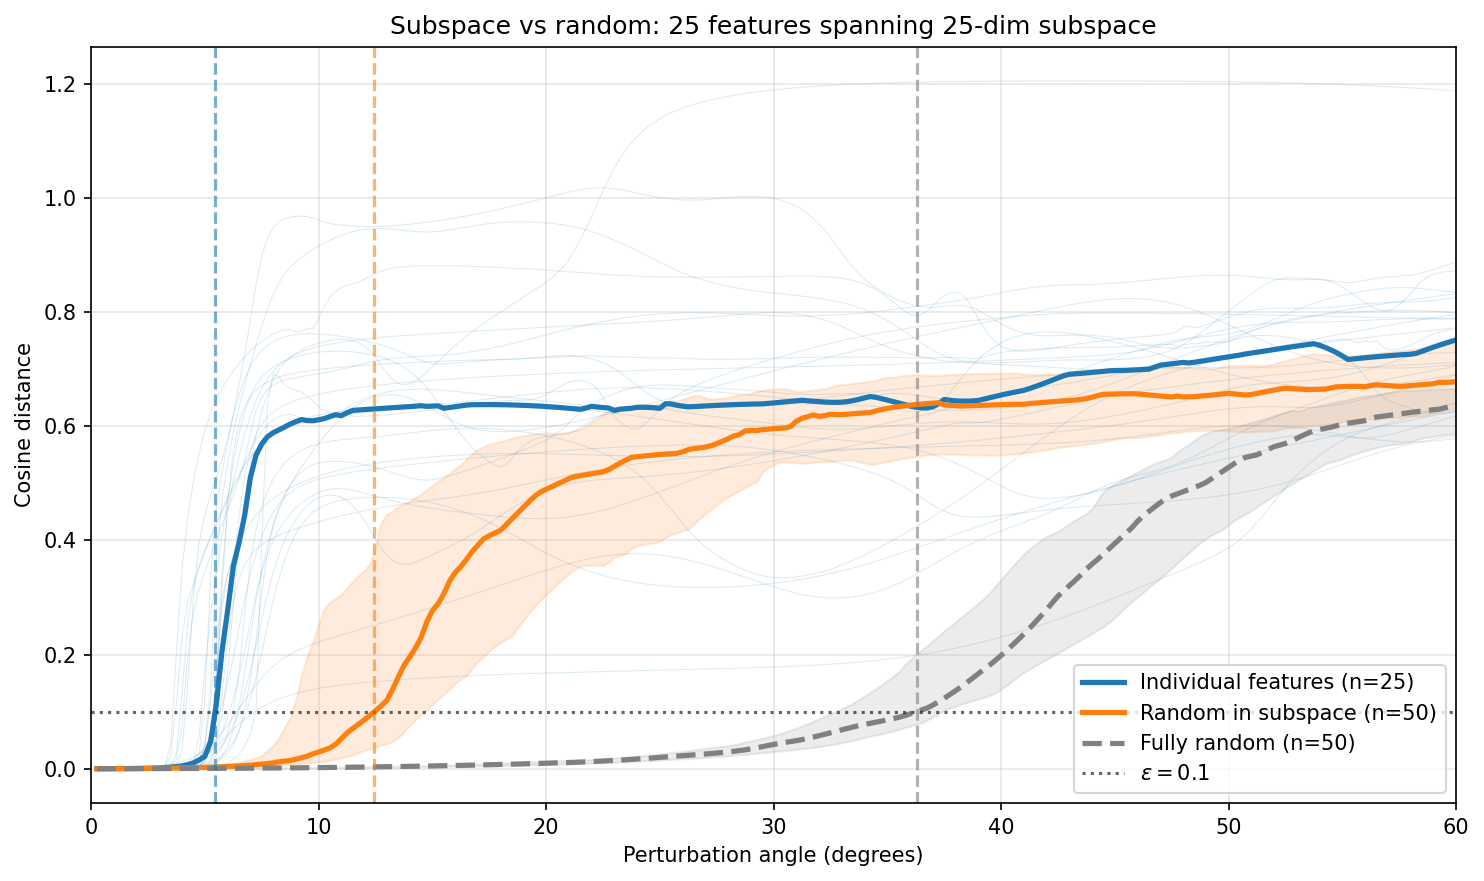
\includegraphics[width=0.7\textwidth]{subspace_vs_random.png}
    \caption{Downstream cosine distance as a function of perturbation angle for three classes of direction: individual features (blue), random directions within the span of 25 known features (orange), and fully random directions (grey). Shaded regions indicate variance across samples. The separation between the three curves is quantitatively predicted by the single-feature dominance model (Equations~\eqref{eq:predicted_break},~\eqref{eq:plateau_breaking_rand}, and~\eqref{eq:plateau_breaking_sub}).}
    \label{fig:subspace_vs_random}
\end{figure}
Individual features break at ${\sim}5.5^\circ$, random directions within the 25-dimensional feature subspace break at ${\sim}12.5^\circ$ (predicted: $11^\circ$), and fully random directions break at ${\sim}36.3^\circ$ (predicted: $36^\circ$ for $m \approx 1{,}000$; note that this is an unusually low feature number given typical assumptions).

\section{Sparsity, superposition, and (tight) frames}
The assumption that features are approximately uniformly spread on the unit sphere can be formalized using the notion of a tight frame.
A collection of vectors $\{f_1, \ldots, f_m\}$ in $\mathbb{R}^n$ forms a \emph{frame} if there exist constants $A, B > 0$ such that $A \|\mathbf{x}\|^2 \leq \sum_i |\langle \mathbf{x}, f_i \rangle|^2 \leq B \|\mathbf{x}\|^2$ for all $\mathbf{x} \in \mathbb{R}^n$.
When $A = B$, the frame is \emph{tight}, which implies that the frame operator $S = \sum_i f_i f_i^\top$ satisfies $S = A I$, where $I$ is the $n \times n$ identity matrix.
For $m$ unit vectors, $A = m/n$.
A tight frame is a natural generalization of an orthonormal basis to the overcomplete setting ($m > n$): reconstruction is straightforward, and features are spread as uniformly as possible across the sphere.
Our assumption that $m \gg n$ features are approximately uniformly spread is therefore the assumption that they form an approximate tight frame.

Given a set of $k$ discovered features, define the partial frame operator $S_k = \sum_{i=1}^k f_i f_i^\top$. If the full feature set is an approximate tight frame, undiscovered features must collectively contribute $S_{\mathrm{missing}} \approx \frac{m}{n} I - S_k$. The low-eigenvalue eigenvectors of $S_k$ therefore indicate directions in activation space where undiscovered features are concentrated, and can be used to initialize further runs of MELBO-like methods.

This diagnostic is only informative when $k$ is large enough that $S_k$ has meaningful spectral structure.
For example, for $k = 25$ in $n = 512$, the operator is heavily rank-deficient and says little beyond ``most of the space is unexplored.'' It becomes useful when $k$ is comparable to or exceeds $n$.

A related observation: as features are discovered in order of decreasing sensitivity, MELBO scores should decrease progressively.
When the optimizer struggles to find new directions above a given plateau-breaking threshold, lowering the threshold should recover additional, weaker features.
At the point where discovery genuinely stalls regardless of threshold, the spectrum of $S_k$ distinguishes two scenarios: a roughly uniform spectrum suggests the discoverable features have been found and the model's feature set at that layer does not span $\mathbb{R}^n$, while a non-uniform spectrum suggests features remain in the underrepresented subspaces.

The tight frame assumption also predicts that the optimal readout direction for a feature (dual frame element $\tilde{f}_i = S^{-1} f_i$) should be approximately proportional to the feature direction itself.
If learned linear probes diverge significantly from MELBO directions, this indicates the feature geometry is far from a tight frame.
This is testable once enough features have been discovered to make $S_k$ well-conditioned.
\end{document}